\documentclass[svgnames,11pt]{beamer}
\input{/home/tof/Documents/Cozy/latex-include/preambule_commun.tex}
\input{/home/tof/Documents/Cozy/latex-include/preambule_beamer.tex}
%\usepackage{pgfpages} \setbeameroption{show notes on second screen=left}
\author[]{Christophe Viroulaud}
\title{Arbre binaire de recherche}
\date{\framebox{\textbf{Algo 09}}}
%\logo{}
\institute{Terminale - NSI}

\begin{document}
\begin{frame}
    \titlepage
\end{frame}
\begin{frame}
    \frametitle{}
    La recherche d'un élément dans un tableau est \textbf{linéaire} dans le pire des cas: elle dépend de la taille du tableau.

    \begin{center}
        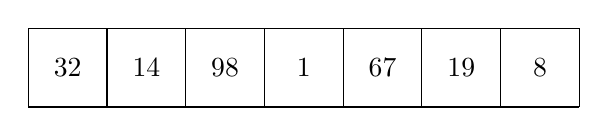
\begin{tikzpicture}
            \draw (0,0) grid (7,1);
            \node (0) at (0.5,0.5) {32};
            \node (1) at (1.5,0.5) {14};
            \node (2) at (2.5,0.5) {98};
            \node (3) at (3.5,0.5) {1};
            \node (4) at (4.5,0.5) {67};
            \node (5) at (5.5,0.5) {19};
            \node (5) at (6.5,0.5) {8};

        \end{tikzpicture}
    \end{center}
\end{frame}
\begin{frame}
    \frametitle{}

    \begin{framed}
        \centering Comment obtenir une méthode de recherche efficace avec les arbres?
    \end{framed}

\end{frame}
\section{Arbre binaire de recherche}
\subsection{Définition}
\begin{frame}
    \frametitle{Arbre binaire de recherche - définition}

    On impose une contrainte à chaque nœud d'un arbre binaire:
    \begin{itemize}
        \item les valeurs du sous-arbre gauche sont plus petites que celle du nœud,
        \item les valeurs du sous-arbre droit sont plus grandes que celle du nœud.
    \end{itemize}
\end{frame}

\begin{frame}
    \frametitle{}


    \begin{center}
        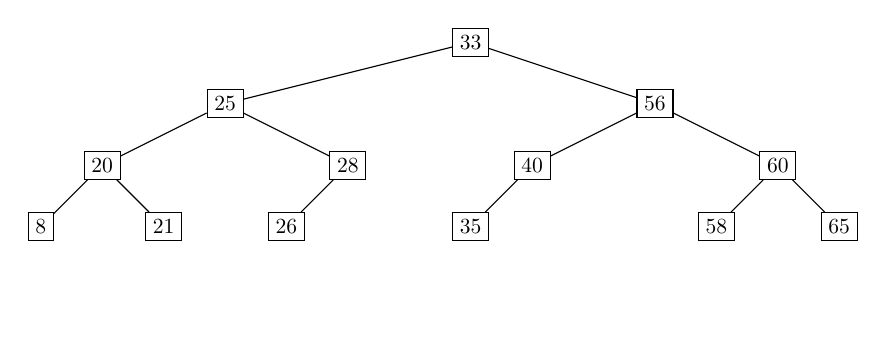
\begin{tikzpicture}[scale=0.78, transform shape]
            \node[draw] (A) at (1,0) {33};
            \node[draw] (B) at (-3,-1) {25};
            \node[draw] (C) at (-5,-2) {20};
            \node[draw] (D) at (-1,-2) {28};
            \node[draw] (E) at (-6,-3) {8};
            \node[draw] (F) at (-4,-3) {21};
            \node[draw] (H) at (-2,-3) {26};
            \node[draw] (I) at (4,-1) {56};
            \node[draw] (J) at (2,-2) {40};
            \node[draw] (K) at (6,-2) {60};
            \node[draw] (M) at (1,-3) {35};
            \node[draw] (O) at (5,-3) {58};
            \node[draw] (P) at (7,-3) {65};

            \draw (A) -- (B);
            \draw (C) -- (B);
            \draw (C) -- (E);
            \draw (C) -- (F);
            \draw (D) -- (B);
            \draw (D) -- (H);
            \draw (A) -- (I);
            \draw (J) -- (I);
            \draw (I) -- (K);
            \draw (J) -- (M);
            \draw (K) -- (O);
            \draw (K) -- (P);
            \draw [white] (0,-3) -- (0,-4.5);
        \end{tikzpicture}
        \captionof{figure}{Un Arbre Binaire de Recherche (\emph{ABR})}
        \label{arbre}
    \end{center}
    \begin{aretenir}[Remarque]
        On suppose que chaque valeur n'apparaît qu'une seule fois dans l'arbre.
    \end{aretenir}

\end{frame}
\begin{frame}
    \frametitle{}

    \begin{activite}
        \begin{enumerate}
            \item Placer les valeurs 23, 27, 54, 55 dans l'ABR.
            \item Où se trouve la plus grande valeur ? La plus petite?
            \item Effectuer un parcours infixe de l'arbre. Que remarque-t-on ?
        \end{enumerate}
    \end{activite}

\end{frame}
\begin{frame}
    \frametitle{Correction}


    \begin{center}
        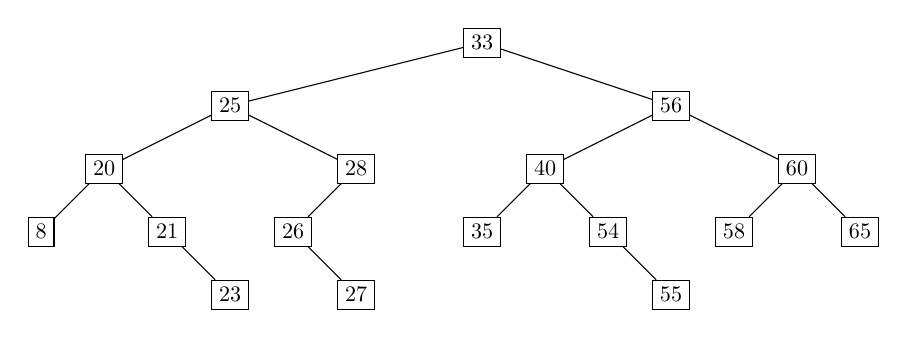
\begin{tikzpicture}[scale=0.8, transform shape]
            \node[draw] (A) at (1,0) {33};
            \node[draw] (B) at (-3,-1) {25};
            \node[draw] (C) at (-5,-2) {20};
            \node[draw] (D) at (-1,-2) {28};
            \node[draw] (E) at (-6,-3) {8};
            \node[draw] (F) at (-4,-3) {21};
            \node[draw] (H) at (-2,-3) {26};
            \node[draw] (I) at (4,-1) {56};
            \node[draw] (J) at (2,-2) {40};
            \node[draw] (K) at (6,-2) {60};
            \node[draw] (M) at (1,-3) {35};
            \node[draw] (O) at (5,-3) {58};
            \node[draw] (P) at (7,-3) {65};
            \node[draw] (Q) at (-3,-4) {23};
            \node[draw] (R) at (-1,-4) {27};
            \node[draw] (S) at (3,-3) {54};
            \node[draw] (T) at (4,-4) {55};


            \draw (A) -- (B);
            \draw (C) -- (B);
            \draw (C) -- (E);
            \draw (C) -- (F);
            \draw (D) -- (B);
            \draw (D) -- (H);
            \draw (A) -- (I);
            \draw (J) -- (I);
            \draw (I) -- (K);
            \draw (J) -- (M);
            \draw (K) -- (O);
            \draw (K) -- (P);
            \draw (F) -- (Q);
            \draw (H) -- (R);
            \draw (J) -- (S);
            \draw (S) -- (T);
        \end{tikzpicture}
        \captionof{figure}{Activité 1}
        \label{arbre}
    \end{center}

\end{frame}
\begin{frame}
    \frametitle{}
    \begin{center}
        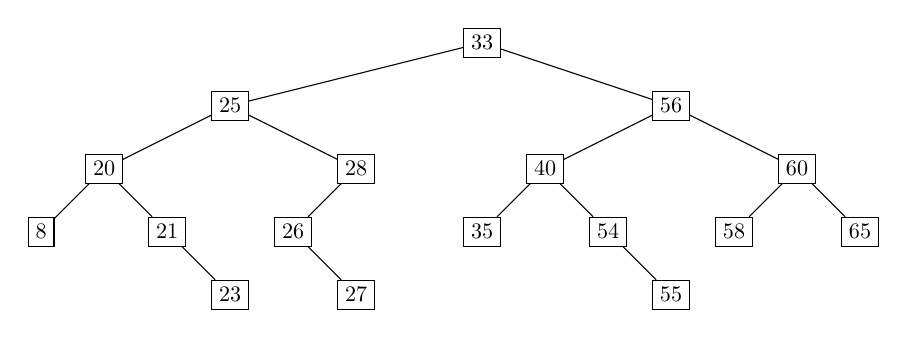
\begin{tikzpicture}[scale=0.8, transform shape]
            \node[draw] (A) at (1,0) {33};
            \node[draw] (B) at (-3,-1) {25};
            \node[draw] (C) at (-5,-2) {20};
            \node[draw] (D) at (-1,-2) {28};
            \node[draw] (E) at (-6,-3) {8};
            \node[draw] (F) at (-4,-3) {21};
            \node[draw] (H) at (-2,-3) {26};
            \node[draw] (I) at (4,-1) {56};
            \node[draw] (J) at (2,-2) {40};
            \node[draw] (K) at (6,-2) {60};
            \node[draw] (M) at (1,-3) {35};
            \node[draw] (O) at (5,-3) {58};
            \node[draw] (P) at (7,-3) {65};
            \node[draw] (Q) at (-3,-4) {23};
            \node[draw] (R) at (-1,-4) {27};
            \node[draw] (S) at (3,-3) {54};
            \node[draw] (T) at (4,-4) {55};


            \draw (A) -- (B);
            \draw (C) -- (B);
            \draw (C) -- (E);
            \draw (C) -- (F);
            \draw (D) -- (B);
            \draw (D) -- (H);
            \draw (A) -- (I);
            \draw (J) -- (I);
            \draw (I) -- (K);
            \draw (J) -- (M);
            \draw (K) -- (O);
            \draw (K) -- (P);
            \draw (F) -- (Q);
            \draw (H) -- (R);
            \draw (J) -- (S);
            \draw (S) -- (T);
        \end{tikzpicture}
        \captionof{figure}{Activité 1}
        \label{arbre}
    \end{center}
    \begin{itemize}
        \item La plus petite valeur est dans le nœud le plus à gauche.
        \item La plus grande valeur est dans le nœud le plus à droite.
        \item parcours infixe: 8 - 20 - 21 - 23 - 25 - 26 - 27 - 28 - 33 - 35 - 40 - 54 - 55 - 56 - 58 - 60 - 65
    \end{itemize}

\end{frame}
\begin{frame}
    \frametitle{}
    \begin{center}
        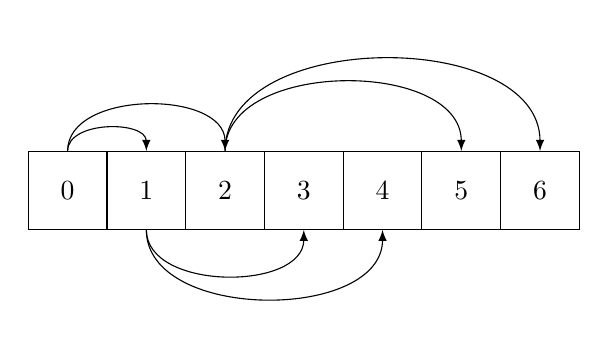
\begin{tikzpicture}
            \draw (0,0) grid (7,1);
            \node (0) at (0.5,0.5) {0};
            \node (1) at (1.5,0.5) {1};
            \node (2) at (2.5,0.5) {2};
            \node (3) at (3.5,0.5) {3};
            \node (4) at (4.5,0.5) {4};
            \node (5) at (5.5,0.5) {5};
            \node (5) at (6.5,0.5) {6};

            \draw[->,>=latex] (0.5,1) to[bend left=90] (1.5,1);
            \draw[->,>=latex] (0.5,1) to[bend left=90] (2.5,1);
            \draw[->,>=latex] (1.5,0) to[bend left=-90] (3.5,0);
            \draw[->,>=latex] (1.5,0) to[bend left=-90] (4.5,0);
            \draw[->,>=latex] (2.5,1) to[bend left=90] (5.5,1);
            \draw[->,>=latex] (2.5,1) to[bend left=90] (6.5,1);

        \end{tikzpicture}
    \end{center}
    \begin{activite}
        Il est judicieux d'utiliser un tableau pour représenter un arbre binaire de recherche.\\Construire par compréhension un tableau \textbf{\texttt{arbre}} rempli de cent 0. On considérera dans la suite, que la valeur 0 représente un nœud vide.
    \end{activite}

\end{frame}
\begin{frame}[fragile]
    \frametitle{Correction}

    \begin{center}
        \begin{lstlisting}[language=Python , basicstyle=\ttfamily\small, xleftmargin=2em, xrightmargin=2em]
arbre = [0 for _ in range(100)]
\end{lstlisting}
    \end{center}

\end{frame}
\subsection{Hauteur}
\begin{frame}
    \frametitle{Hauteur}

    \begin{center}
        {\Large $$h+1 \leq n \leq 2^{h+1}-1$$    }
        \captionof{code}{Propriété des arbres binaires}
    \end{center}
\end{frame}
\begin{frame}
    \frametitle{Nouvelle propriété}
    {\Large $$2^h  \leq n \leq 2^{h+1}-1$$    }
    Car il y a entre 1 et $2^h$ nœuds sur le dernier niveau.
    \begin{center}
        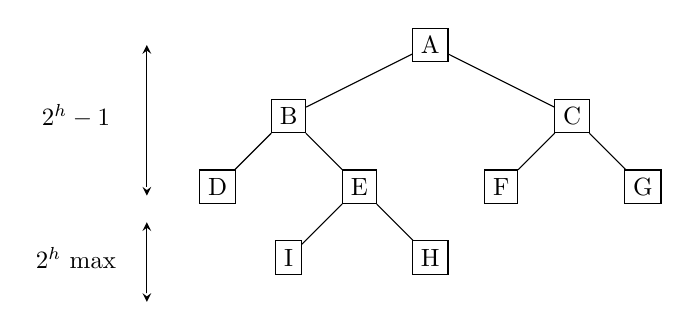
\begin{tikzpicture}[scale=0.9, transform shape]
            \node[draw] (1) at (0,0) {A};
            \node[draw] (2) at (-2,-1) {B};
            \node[draw] (3) at (2,-1) {C};
            \node[draw] (4) at (-3,-2) {D};
            \node[draw] (5) at (-1,-2) {E};
            \node[draw] (6) at (1,-2) {F};
            \node[draw] (7) at (3,-2) {G};
            \node[draw] (8) at (0,-3) {H};
            \node[draw] (9) at (-2,-3) {I};

            \draw (1) -- (2);
            \draw (1) -- (3);
            \draw (2) -- (4);
            \draw (2) -- (5);
            \draw (3) -- (6);
            \draw (3) -- (7);
            \draw (5) -- (8);
            \draw (5) -- (9);
            \node at(-5,-1){$2^{h}-1$ };
            \draw[stealth-stealth reversed] (-4,0) |- (-4,-2);
            \node at(-5,-3){$2^{h}$ max };
            \draw[stealth-stealth reversed] (-4,-2.5) |- (-4,-3.5);
        \end{tikzpicture}
    \end{center}
\note{1 nœud au moins sur dernier niveau d'où $2^h$ dans 1° inégalité}
\end{frame}
\begin{frame}
    \frametitle{}

    {\Large $$2^h  \leq n \leq 2^{h+1}-1$$    }
    {\Large $$\Rightarrow 2^h  \leq n \leq 2^{h+1} $$    }
    {\Large $$\Leftrightarrow h  \leq \log_2 (n) \leq h+1 $$    }
    \begin{aretenir}[]
        Dans un arbre binaire \textbf{équilibré}:
        {\Large $$h = \log_2(n)$$}
    \end{aretenir}
\end{frame}
\begin{frame}
    \frametitle{}

    \begin{aretenir}[Hors programme]
        On peut rééquilibrer un arbre en effectuant des \textbf{rotations}.
    \end{aretenir}

\end{frame}
\subsection{Insertion}
\begin{frame}
    \frametitle{Insertion}

    Pour insérer un élément dans un arbre binaire de recherche:
    \begin{itemize}
        \item On part de la racine.
        \item On descend dans le sous-arbre gauche si l'élément est inférieur à la racine.
        \item On descend dans le sous-arbre droit si l'élément est supérieur à la racine.
    \end{itemize}
    On applique récursivement cet algorithme jusqu'à une feuille.
\end{frame}
\begin{frame}
    \frametitle{}

    \begin{center}
        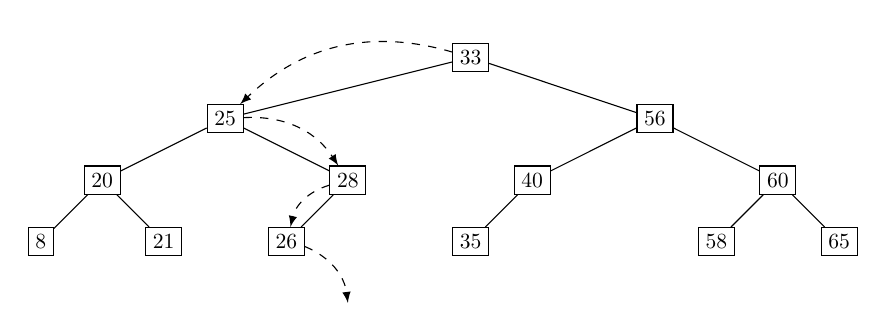
\begin{tikzpicture}[scale=0.78, transform shape]
            \node[draw] (A) at (1,0) {33};
            \node[draw] (B) at (-3,-1) {25};
            \node[draw] (C) at (-5,-2) {20};
            \node[draw] (D) at (-1,-2) {28};
            \node[draw] (E) at (-6,-3) {8};
            \node[draw] (F) at (-4,-3) {21};
            \node[draw] (H) at (-2,-3) {26};
            \node[draw] (I) at (4,-1) {56};
            \node[draw] (J) at (2,-2) {40};
            \node[draw] (K) at (6,-2) {60};
            \node[draw] (M) at (1,-3) {35};
            \node[draw] (O) at (5,-3) {58};
            \node[draw] (P) at (7,-3) {65};

            \draw (A) -- (B);
            \draw (C) -- (B);
            \draw (C) -- (E);
            \draw (C) -- (F);
            \draw (D) -- (B);
            \draw (D) -- (H);
            \draw (A) -- (I);
            \draw (J) -- (I);
            \draw (I) -- (K);
            \draw (J) -- (M);
            \draw (K) -- (O);
            \draw (K) -- (P);
            \draw[->,>=latex, dashed] (A) to[bend right] (B);
            \draw[->,>=latex, dashed] (B) to[bend left] (D);
            \draw[->,>=latex, dashed] (D) to[bend right] (H);
            \draw[->,>=latex, dashed] (H) to[bend left] (-1,-4);
        \end{tikzpicture}
        \captionof{figure}{Ajouter 27}
        \label{arbre}
    \end{center}

\end{frame}
\begin{frame}
    \frametitle{}

    \begin{activite}
        \begin{enumerate}
            \item Quelle est la complexité temporelle de cet algorithme?
            \item Écrire la fonction récursive \textbf{\texttt{inserer(val: int, abr: list, i\_pere: int) $\rightarrow$ None}} qui insère \textbf{\texttt{val}} dans l'arbre de recherche \textbf{\texttt{abr}} représenté par un tableau.
            \item Insérer dans l'ordre les valeurs: 33, 56, 25, 20, 28, 40, 21, 8, 26, 60, 35, 58, 65.
        \end{enumerate}
    \end{activite}

\end{frame}
\begin{frame}[fragile]
    \frametitle{Correction}

    \begin{center}
        \begin{lstlisting}[language=Python , basicstyle=\ttfamily\small, xleftmargin=.5em, xrightmargin=-1em]
def inserer(val: int, abr: list, i_pere: int) -> None:
    if abr[i_pere] == 0:  # cellule vide: cas limite
        abr[i_pere] = val
    elif val < abr[i_pere]:
        inserer(val, abr, 2*i_pere+1)  # gauche
    else:
        inserer(val, abr, 2*i_pere+2)  # droite
\end{lstlisting}
    \end{center}
    \begin{aretenir}[]
        L'insertion a une complexité logarithmique $O(\log_2(n))$. On parcourt au maximum la hauteur de l'arbre.
    \end{aretenir}
\end{frame}
\begin{frame}[fragile]
    \frametitle{}

    \begin{center}
        \begin{lstlisting}[language=Python , basicstyle=\ttfamily\small, xleftmargin=2em, xrightmargin=2em]
inserer(33, arbre, 0)
inserer(56, arbre, 0)
inserer(25, arbre, 0)
...
\end{lstlisting}
    \end{center}
    \begin{aretenir}[Remarque]
        Selon l'ordre d'ajout, l'arbre produit ne sera pas le même.
    \end{aretenir}
\end{frame}
\subsection{Recherche}
\begin{frame}
    \frametitle{Recherche}

    Pour rechercher un élément dans un arbre binaire de recherche:
    \begin{itemize}
        \item On part de la racine.
        \item On descend dans le sous-arbre gauche si l'élément est inférieur à la racine.
        \item On descend dans le sous-arbre droit si l'élément est supérieur à la racine.
    \end{itemize}
    On applique récursivement cet algorithme jusqu'à trouver l'élément ou bien arriver à une feuille.

\end{frame}
\begin{frame}[fragile]
    \begin{center}
        \begin{lstlisting}[language=Python , basicstyle=\ttfamily\small, xleftmargin=0.5em, xrightmargin=-1em]
[33, 25, 56, 20, 28, 40, 60, 8, 21, 26, 35, 58, 65]
\end{lstlisting}
    \end{center}
    \begin{center}
        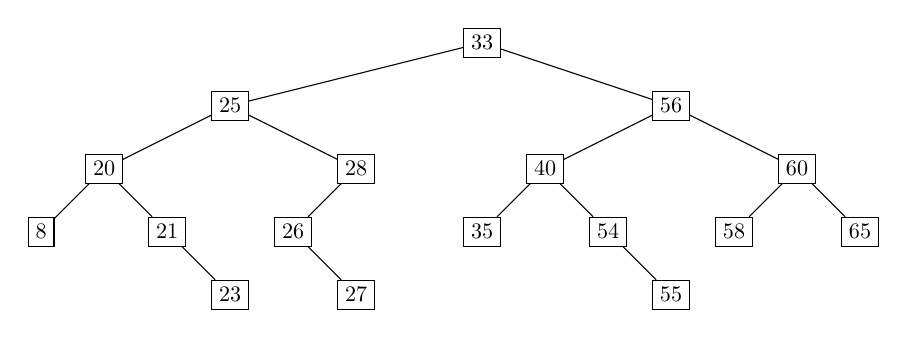
\begin{tikzpicture}[scale=0.8, transform shape]
            \node[draw] (A) at (1,0) {33};
            \node[draw] (B) at (-3,-1) {25};
            \node[draw] (C) at (-5,-2) {20};
            \node[draw] (D) at (-1,-2) {28};
            \node[draw] (E) at (-6,-3) {8};
            \node[draw] (F) at (-4,-3) {21};
            \node[draw] (H) at (-2,-3) {26};
            \node[draw] (I) at (4,-1) {56};
            \node[draw] (J) at (2,-2) {40};
            \node[draw] (K) at (6,-2) {60};
            \node[draw] (M) at (1,-3) {35};
            \node[draw] (O) at (5,-3) {58};
            \node[draw] (P) at (7,-3) {65};
            \node[draw] (Q) at (-3,-4) {23};
            \node[draw] (R) at (-1,-4) {27};
            \node[draw] (S) at (3,-3) {54};
            \node[draw] (T) at (4,-4) {55};


            \draw (A) -- (B);
            \draw (C) -- (B);
            \draw (C) -- (E);
            \draw (C) -- (F);
            \draw (D) -- (B);
            \draw (D) -- (H);
            \draw (A) -- (I);
            \draw (J) -- (I);
            \draw (I) -- (K);
            \draw (J) -- (M);
            \draw (K) -- (O);
            \draw (K) -- (P);
            \draw (F) -- (Q);
            \draw (H) -- (R);
            \draw (J) -- (S);
            \draw (S) -- (T);
        \end{tikzpicture}
    \end{center}
    \begin{activite}
        \begin{enumerate}
            \item Quelle la complexité temporelle dans le pire des cas de la recherche d'un élément dans le tableau?
            \item Que devient cette complexité pour un arbre binaire de recherche?
        \end{enumerate}
    \end{activite}
\end{frame}
\begin{frame}
    \frametitle{Correction}

    \begin{itemize}
        \item Dans un tableau la recherche a une complexité \textbf{linéaire, $O(n)$}.
        \item Dans un ABR la recherche a une complexité \textbf{logarithmique, $O(\log_2(n))$} dans le pire des cas (c'est à dire quand on ne trouve pas l'élément).
    \end{itemize}

\end{frame}
\begin{frame}
    \begin{activite}
        Écrire la fonction récursive \textbf{\texttt{rechercher(val: int, abr: list, i\_pere: int) $\rightarrow$ bool}} qui cherche si \textbf{\texttt{val}} est présent dans l'arbre \textbf{\texttt{abr}}.
    \end{activite}


\end{frame}
\begin{frame}[fragile]
    \frametitle{Correction}

    \begin{center}
        \begin{lstlisting}[language=Python , basicstyle=\ttfamily\small, xleftmargin=0.5em, xrightmargin=-3em]
def rechercher(val: int, abr: list, i_pere: int) -> bool:
    if abr[i_pere] == 0: # non trouvé
        return False
    elif abr[i_pere] == val: # trouvé
        return True
    elif val < abr[i_pere]: # gauche
        return rechercher(val, abr, 2*i_pere+1)
    else: # droit
        return rechercher(val, abr, 2*i_pere+2)
\end{lstlisting}
    \end{center}

\end{frame}
\begin{frame}
    \frametitle{}

    \begin{itemize}
        \item<1-> Considérons un arbre binaire de recherche qui contient 1 million d'éléments.
        \item<2-> Sa hauteur est $h\simeq \log_2(1000000)\simeq 20$
        \item<3-> Il faut seulement 20 étapes pour effectuer une recherche dans l'arbre, contre 1 million dans un tableau.
    \end{itemize}
\end{frame}
\end{document}